\documentclass[12pt, answers]{exam} % Clase para exámenes con respuestas
\usepackage{amsmath, amssymb} % Paquetes para matemáticas avanzadas
\usepackage{graphicx} % Inclusión de gráficos
\usepackage{tikz} % Dibujos y figuras en LaTeX
\usepackage{enumitem} % Listas personalizadas
\usepackage[letterpaper, top=2cm, bottom=2cm, left=3cm, right=3cm]{geometry} % Configuración de márgenes

% Configuración de encabezado y pie de página
\pagestyle{headandfoot}
\firstpageheader{Examen de Física}{}{} 
\runningheader{Examen de Física}{}{}
\firstpagefooter{}{\thepage}{}
\runningfooter{}{\thepage}{}

% Configuración del título de las respuestas
\renewcommand{\solutiontitle}{\noindent\textbf{Respuesta:}\par\noindent}

\begin{document}

\begin{center}
    \large\textbf{Examen de Física}\\[1em]
    \large Ingeniería Física, Segundo Ciclo\\[1em]
\end{center}

\begin{questions}

    % Pregunta 1
    \question \large\textbf{Dos esferas de masa 1gr y de igual carga Q se cuelgan de hilos de 20cm y masa despreciable sujetos a un mismo punto. Si el ángulo que forman los hilos en el punto común es de 20°, calcular el valor de Q.}

    
        El sistema consiste en dos esferas en equilibrio debido a la fuerza eléctrica y la tensión del hilo, equilibrando la gravedad. Descomponemos las fuerzas:
    
        \[
        F_g = m \cdot g = 0.001 \cdot 9.8 \, \text{N}
        \]
    
        La componente horizontal de la tensión es igual a la fuerza eléctrica:
        \[
        T \cdot \sin(\theta) = F_e = k \frac{Q^2}{r^2}
        \]
        La componente vertical de la tensión equilibra el peso:
        \[
        T \cdot \cos(\theta) = m \cdot g
        \]
    
        Dividiendo ambas ecuaciones:
        \[
        \frac{\sin(\theta)}{\cos(\theta)} = \frac{F_e}{F_g} \quad \Rightarrow \quad \tan(\theta) = \frac{k \frac{Q^2}{r^2}}{m \cdot g}
        \]
    
        Resolviendo para $Q$:
        \[
        Q = \sqrt{\frac{r^2 \cdot m \cdot g \cdot \tan(\theta)}{k}}
        \]
    
        Ahora, calculamos los valores. Para $r = 0.2 \, \text{m} \cdot \sin(10^\circ)$ y $\theta = 10^\circ$:
        
        \[
        r = 0.2 \, \text{m}, \, \theta = 10^\circ, \, m = 0.001 \, \text{kg}, \, k = 9 \times 10^9 \, \text{Nm}^2/\text{C}^2
        \]
        
        \[
        Q \approx \sqrt{\frac{(0.2)^2 \cdot 0.001 \cdot 9.8 \cdot \tan(10^\circ)}{9 \times 10^9}}
        \]
  
    
        \vspace{1cm}
        
        % TikZ Diagram
      \begin{center}
        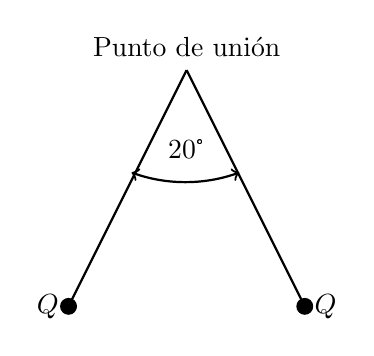
\begin{tikzpicture}
            % Drawing the spheres
            \draw[fill=black] (-1.5, 0) circle (0.1) node[left] {$Q$};
            \draw[fill=black] (1.5, 0) circle (0.1) node[right] {$Q$};
    
            % Drawing the threads
            \draw[thick] (0,3) -- (-1.5,0);
            \draw[thick] (0,3) -- (1.5,0);
    
            % Drawing the angle
            \draw[<->, thick] (-0.7,1.7) arc[start angle=-110, end angle=-70, radius=2];
            \node at (0,2) {20°};
    
            % Labels
            \node at (0,3.3) {Punto de unión};
        \end{tikzpicture}
      \end{center}
    

    % Pregunta 2
    \question \large\textbf{Calcular el campo eléctrico producido por un alambre de 2 m de longitud ubicado en la dirección del eje x, y cargado con una densidad lineal de carga dada por $\lambda = (x^2 + 2)$C/m en un punto a 0.5 m del extremo del alambre sobre el mismo eje x.}

    
        Para calcular el campo eléctrico en un punto ubicado a \( 0.5 \, \text{m} \) del extremo del alambre, utilizamos la ley de Coulomb para un elemento de carga \( dq \) sobre el alambre. La densidad lineal de carga es \( \lambda = (x^2 + 2) \, \text{C/m} \), por lo que un elemento infinitesimal de carga es:
        
        \[
        dq = \lambda \, dx = (x^2 + 2) \, dx
        \]
        
        El campo eléctrico en el punto \( P \) a una distancia de \( 0.5 \, \text{m} \) del extremo del alambre es la suma de los campos creados por cada elemento de carga. Aplicando la fórmula para el campo eléctrico:
        
        \[
        dE = \frac{1}{4 \pi \epsilon_0} \cdot \frac{dq}{r^2}
        \]
        
        donde \( r \) es la distancia entre el elemento de carga y el punto \( P \). Integramos a lo largo de la longitud del alambre (desde \( x = 0 \) hasta \( x = 2 \, \text{m} \)):
        
        \[
        E = \frac{1}{4 \pi \epsilon_0} \int_0^2 \frac{(x^2 + 2) \, dx}{(x + 0.5)^2}
        \]
        
        Calculamos el resultado de la integral numéricamente para obtener el valor del campo eléctrico en \( P \).

    % Pregunta 3
    \question \large\textbf{¿Cuál es la intensidad del campo eléctrico en el interior de una esfera maciza cargada? ¿Y si esta fuera hueca? ¿Y si además la esfera fuera conductora?}

    
        Para una esfera maciza cargada uniformemente, aplicamos la ley de Gauss. El campo eléctrico en un punto dentro de la esfera, a una distancia \( r \) del centro, se determina considerando una superficie gaussiana esférica de radio \( r \). Según la ley de Gauss, tenemos:
        
        \[
        \oint \vec{E} \cdot d\vec{A} = \frac{q_{\text{enc}}}{\epsilon_0}
        \]
        
        El campo eléctrico en el interior de la esfera maciza es:
        
        \[
        E = \frac{1}{4 \pi \epsilon_0} \frac{Q r}{R^3}, \text{ para } r < R
        \]
        
        donde \( Q \) es la carga total de la esfera, \( r \) es la distancia al centro de la esfera y \( R \) es el radio de la esfera.
        
        Si la esfera es hueca, no hay carga dentro de la superficie gaussiana, y el campo eléctrico en el interior es cero:
        
        \[
        E = 0, \text{ para } r < R \text{ (esfera hueca)}
        \]
        
        Si la esfera es conductora, la carga reside en la superficie exterior y el campo eléctrico en el interior también es cero:
        
        \[
        E = 0, \text{ para } r < R \text{ (esfera conductora)}
        \]
        
        
     \begin{center}
           % TikZ Picture
           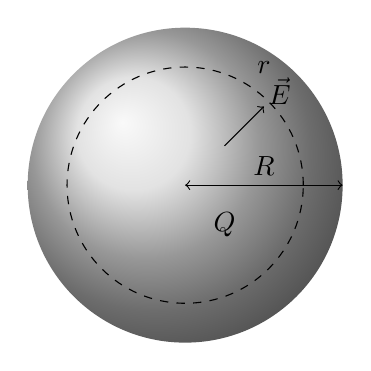
\begin{tikzpicture}
            % Esfera maciza
            \shade[ball color = gray!30] (0,0) circle (2);
            
            % Radio R
            \draw[<->] (0,0) -- (2,0) node[midway, above] {$R$};
            
            % Superficie gaussiana
            \draw[dashed] (0,0) circle (1.5);
            \node at (1,1.5) {$r$};
            
            % Carga distribuida
            \node at (0.5,-0.5) {$Q$};
            
            % Campo en el interior
            \draw[->] (0.5,0.5) -- (1,1);
            \node at (1.2,1.2) {$\vec{E}$};
        \end{tikzpicture}
     \end{center}
        

    % Pregunta 4
    \question \large\textbf{Dos cargas puntuales de 5C y -5C ubicadas en los puntos (1,1) m y (5,5) m. Calcular el potencial en el punto (5,0). Sugerencia: aplicar el principio de superposición.}

   
        El potencial eléctrico en un punto debido a una carga puntual \( q \) se calcula como:
        
        \[
        V = \frac{1}{4 \pi \epsilon_0} \cdot \frac{q}{r}
        \]
        
        Aplicando el principio de superposición, el potencial total en el punto \( (5,0) \) es la suma de los potenciales debidos a las dos cargas \( 5 \, \text{C} \) y \( -5 \, \text{C} \).
        
        - La distancia desde el punto \( (5,0) \) a la carga \( 5 \, \text{C} \) ubicada en \( (1,1) \, \text{m} \) es:
        
        \[
        r_1 = \sqrt{(5-1)^2 + (0-1)^2} = \sqrt{16 + 1} = \sqrt{17} \, \text{m}
        \]
        
        - La distancia desde el punto \( (5,0) \) a la carga \( -5 \, \text{C} \) ubicada en \( (5,5) \, \text{m} \) es:
        
        \[
        r_2 = \sqrt{(5-5)^2 + (0-5)^2} = 5 \, \text{m}
        \]
        
        El potencial total en el punto \( (5,0) \) es:
        
        \[
        V = \frac{1}{4 \pi \epsilon_0} \left( \frac{5}{\sqrt{17}} + \frac{-5}{5} \right)
        \]
        
        Resolviendo:
        
        \[
        V = \frac{1}{4 \pi \epsilon_0} \left( \frac{5}{\sqrt{17}} - 1 \right)
        \]
        
        
        
        % TikZ Picture
        \begin{tikzpicture}
            % Ejes coordenados
            \draw[->] (-1,0) -- (6,0) node[anchor=north] {$x$};
            \draw[->] (0,-1) -- (0,6) node[anchor=east] {$y$};
        
            % Cargas puntuales
            \draw[fill=black] (1,1) circle (0.05) node[anchor=east] {$5C$};
            \draw[fill=black] (5,5) circle (0.05) node[anchor=west] {$-5C$};
        
            % Punto (5,0)
            \draw[fill=red] (5,0) circle (0.05) node[anchor=north] {$(5,0)$};
        
            % Distancias
            \draw[dashed] (1,1) -- (5,0);
            \draw[dashed] (5,5) -- (5,0);
            
            % Etiquetas de distancia
            \node at (3.2,0.7) {$r_1 = \sqrt{17}$};
            \node at (5.2,2.5) {$r_2 = 5$};
        \end{tikzpicture}
        

    % Pregunta 5
    \question \large\textbf{¿Cuál es la energía potencial eléctrica que tiene el Sistema del ejercicio anterior?}

    
        La energía potencial eléctrica de un sistema de dos cargas puntuales se calcula como:
        
        \[
        U = \frac{1}{4 \pi \epsilon_0} \cdot \frac{q_1 q_2}{r}
        \]
        
        Donde:
        - \( q_1 = 5 \, \text{C} \)
        - \( q_2 = -5 \, \text{C} \)
        - \( r \) es la distancia entre las dos cargas, que es:
        
        \[
        r = \sqrt{(5-1)^2 + (5-1)^2} = \sqrt{16 + 16} = \sqrt{32} = 4\sqrt{2} \, \text{m}
        \]
        
        Sustituyendo los valores:
        
        \[
        U = \frac{1}{4 \pi \epsilon_0} \cdot \frac{(5)(-5)}{4\sqrt{2}} = \frac{-25}{4 \pi \epsilon_0 4\sqrt{2}} \, \text{J}
        \]
        
        Por lo tanto, la energía potencial del sistema es negativa debido a la interacción de cargas opuestas y tiene un valor de:
        
        \[
        U = \frac{-25}{4 \pi \epsilon_0 4\sqrt{2}} \, \text{J}
        \]
        
        
        % TikZ Picture
        \begin{tikzpicture}
            % Ejes coordenados
            \draw[->] (-1,0) -- (6,0) node[anchor=north] {$x$};
            \draw[->] (0,-1) -- (0,6) node[anchor=east] {$y$};
        
            % Cargas puntuales
            \draw[fill=black] (1,1) circle (0.05) node[anchor=east] {$5C$};
            \draw[fill=black] (5,5) circle (0.05) node[anchor=west] {$-5C$};
        
            % Distancia entre las cargas
            \draw[dashed] (1,1) -- (5,5);
        
            % Etiqueta de distancia
            \node at (3,3.7) {\text{r}};
        \end{tikzpicture}
        
\end{questions}

\end{document}
